%-------------------------------------------------------------------------------
\section{Introduction}
%-------------------------------------------------------------------------------
Web application developers today have more incentives than ever to provide better privacy for their
users.
%
Laws like the EU's General Data Protection Regulation (GDPR)~\cite{eu:gdpr} and California's
Consumer Privacy Act (CCPA)~\cite{ca:privacy-act} codify users' right to be forgotten, and restrict
any data retention to to anonymized information.
%
Legal consequences and the reputational damange associated with data breaches~\cite{breach:amazon,
breach:twitter, breach:fb, breach:marriott, breach:quora} make it good practice to minimize the user
data retained at any point.
%

%
Although many developers are well-intentioned, getting privacy transformations---such as user
unsubscription---right is challenging.
%
They must perform data privacy transformations to adhere to the privacy policy, while ensuring that
the application retains data required for legal purposes or to preserve application utility, and
without violating application invariants.
%
For example, unsubscription of one user should not allow another user to view content that she
originally could not access.

%\lyt{Frans: this paragraph is too abstract, should lead with examples (and then maybe we don't even
%need this?). Also should not apologize for not guaranteeing privacy, but instead enforce that it's
%the developer's job to write the right spec in S3/4.}
%Transformations that achieve better user privacy requires careful handling of data deletion,
%anonymization, and structural decorrelation, where developers must consider how to handle both
%clearly identifying content (\eg usernames), and also structural correlations between data records
%that can identify the user.
%While these transformations do not enable formal privacy \emph{guarantees}, developers can improve
%the state of privacy in applications today by reasoning about often subtle identifying
%correlations.

Privacy transformations must handle both identifying data content, as well as subtly identifying
correlations between data entities. For example, anonymized public running routes correlated with
the same location can identify the user's hometown and be reassociated with the user;
%anonymized posts on Reddit correlated with a subreddit with very few subscribers can be associated
%back to a single user;
papers' affiliation and reviewer conflicts in HotCRP can reidentify the author; and anonymized order
history can reidentify the buyer.

As privacy policies become more complex, the burden of implementing the corresponding privacy
transformation correctly grows as well.  Consequently, today's applications often support only
coarse-grained and simple privacy policies, implemented using ad-hoc methods.

%We next describe a wide range of privacy transformations, some from existing applications' privacy policies,
%and others that demonstrate the potential for better, more nuanced privacy policies. Implementing
%these transformations using ad-hoc methods places undue labor on the developer and, as policies grow
%more complex, becomes more error-prone.

To systematically address these challenges, we propose \emph{data disguising}, a new framework for
specifying and implementing transformations for privacy policies.
%
With data disguising, developers specify transformations required in privacy policies as high-level \emph{data
disguises}. Applying a disguise transforms the state of application data to, \eg, hide a users'
identifiers.
%
%Disguises consist of transformations performed on the high-level object graph embedded in
%database-based applications (encoded by \eg foreign key relationships in relational
%databases)~\cite{orms}.
%Data masks the state of the object graph embedded in database-based applications (\eg
%encoded by foreign key relationships) after mask application.
%and constrains the state of the object graph embedded in
%database-backed applications (\eg encoded by foreign key relationships).
%
Data disguisers take a disguise and the disguise target, and automatically translates the
disguise into the appropriate database transformations to achieve the disguised state. With
disguisers, developers need to reason only about constraints on the entity graph, and can avoid the
labor of manually implementing the disguise.

\section{The Need for Privacy Transformations}
\label{sec:survey}

%
We surveyed several widely-used web applications to understand what privacy-increasing operations
they apply on user unsubscription.
%
A set of common themes emerged.
%~\cite{facebook:privacy, twitter:privacy, hotcrp:privacy, reddit:privacy,
%github:privacy, hackernews:privacy, strava:privacy, linkedin:privacy, stackoverflow:privacy,
%wikipedia:privacy, amazon:privacy, prestashop:privacy, spotify:privacy, lobsters:privacy}:
%
Some services that publicly display user contributions (\eg Wikipedia~\cite{wikipedia:privacy},
StackOverflow~\cite{stackoverflow:privacy}, Strava~\cite{strava:privacy}) keep them publicly
and indefinitely available even if a user deletes their account.
%
Social networking platforms, which fundamentally thrive off users' \emph{shared} data, keep
contributions directly shared with another user unanonymized and visible to the recipient
(\eg Facebook~\cite{facebook:privacy}, LinkedIn~\cite{linkedin:privacy},
Twitter~\cite{twitter:privacy}).
%
Other platforms with mostly public content keep user contributions visible to the intended
audience, but anonymize them by reattributing the contribution to a placeholder user
(\eg GitHub's @ghost~\cite{github:privacy}, Reddit~\cite{reddit:privacy},
Lobste.rs~\cite{lobsters:privacy}).
%
%    \item Keep certain user contributions unanonymized and visible to its intended audience (\eg
%        HotCRP, Lobsters, Wikipedia, HackerNews~\cite{hotcrp:privacy, lobsters:privacy,
%        hackernews:privacy, wikipedia:privacy}).
%    \item Delete user contributions on user profile or feed (\eg Facebook,
%        Twitter~\cite{facebook:privacy, twitter:privacy}).
%\end{itemize}
%
All applications surveyed retain some personal information for legal or necessary business
purposes.
%
Moreover, all applications apply these operations in an ad-hoc way \ms{what do we mean by this?
can we clarify?} and only on explicit, complete user account deletion (a fairly rare event).
%

%
In this paper, we argue that users, developers, and service operators have much to gain from a
\emph{systematic} treatment of privacy-related data transformations (\emph{privacy
transformations}).
%
In particular, the following policies and concepts are missing from today's applications, but
easily described as a privacy transformation.
%

\paragraph{Nuanced policies.}
%
Users---and application developers---might benefit from more nuanced privacy policies.
%
For example, a confidential paper review system like HotCRP wish to keep user's contributions
(papers, reviews), but associate each contribution with a different user account to avoid
revealing the unsubscribed reviewer's identity.
%
Likewise, user contributions with a shared property (\eg posts on Reddit that share a common
tag) might be removed entirely (to avoid inference attacks), or retained, but decorrelated the
contribution itself from the property (\eg keeping the user's posts on Reddit, but removing
their tags).
%
The same policy might apply, but \emph{only} if the property was created by the user (\eg keeping
the user's posts on Reddit, but removing any user-created tags from the posts), or if the user's
contributions comprise more than $p$ percent of the contributions with a shared property.
%(\eg remove the user's posts on Reddit with tag $t$ if these posts comprise more than 10\%
%of all posts with tag $t$).
%
We could even imagine individual users specifying different policies for their data, and having a
privacy transformation framework turn these into concrete operations when a privacy transformation
is applied.
%

\paragraph{Data decomposition.}
%
Privacy transformations go beyond account deletion.
%
For example, applications could support a data expiration policy that encrypts the user's
profile and anonymizes their contributions after the user has been inactive for a fixed period of
time, and restores the user's profile and contributions if the user ever logs back in.
%
Or an application could gradually ``decompose'' sensitive data by applying a serious of
privacy transformations that incrementally remove more identifiable information from it.
%


\paragraph{Reversibility.}
%
Many applications might wish to employ \emph{reversible} transformations, going beyond permanent
and irrevokable unsubscription.
%
After all, if services must allow users to remove their data on request, it's in the operator's
interest to make it easy for users to change their mind and return.
%
An advanced reversible transformation might, for example, record all actions performed in an
encrypted log, and offer that log for download or push it to third-party cloud storage.
%
If the user wishes to return, they simply supply the log and the transformation reverses.
%
To ensure access to the log even if the user loses their key, the transformation might
secret-share the encryption key~\cite{secretsharing} among the user, the service, and a trusted
third party (\eg the ACLU, or EFF).
%



\section{Data Disguising: A New Approach to Privacy Policies}
%\begin{figure}[t!]
%    \centering
%    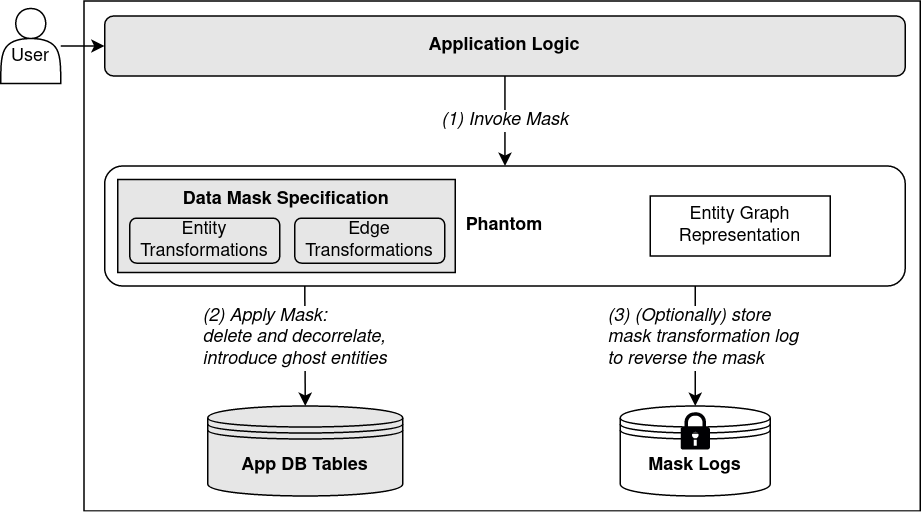
\includegraphics[width=0.5\textwidth]{img/impl}
%
%    \caption{Architecture of \sys, a prototype data disguiser. Developers specify grayed-out components.}
%    \label{fig:arch}
%\end{figure}
\lyt{TODO (Frans): drive w/explicit example of table rows and foreign key relationships, too
abstract. Start with Figure~\ref{fig:arch}?}

To enable developers to better support existing and new privacy policies without onerous manual
labor, we propose \emph{data disguising}.
%
With data disguising, developers specify privacy transformations for database-backed web
applications as high-level, declarative \emph{data disguises}.

A data disguiser sits between application logic and its database. Figure~\ref{fig:arch} shows the
architecture of our prototype, \sys, which works for applications using relational databases.
Disguisers automatically translate the provided disguise into the appropriate database transformations, and
applies them starting at a given disguise target (\eg a row in the users table) when invoked.

Data disguising works on top of the object graph encoded by database-backed
applications~\cite{orm}. In the context of relational databases, the nodes of the object graph are
table rows, and the edges of the object graph are foreign key relationships. Data disguises impose
restrictions on the content and structure of this graph. Unsubscription, for example, transforms
this graph to comply with particular constraints of the privacy transformation for account deletion
by modifying table row contents and rewriting foreign key relationships.

Using their application expertise, the developer selects from a menu of possible transformations
(Section~\ref{sec:policies}) that can be performed on objects and object graph edges.
The data disguise consists of the chosen set of transformations, and determines the
structure of the object graph after a target (\eg the unsubscribing user) is disguised.

Disguising a target object creates \emph{guises}---transformed versions and/or copies of the target.
Disguising requires object deletion and anonymization: guises help maintain referential integrity
when data is deleted, and transform objects into anonymized forms.  Guises additionally decorrelate
other objects from the target: for example, a new guise for the user can be created in the users
table, and the foreign key relationship from a row in the posts table rewritten to point this guise,
to decorrelate the post from the user.

%can expressed via transformations that restructure the entity graph with edges to ghost entities
%that have replaced real ones.

%Data masking tools take a data mask and the top-level entity to mask, and automatically generate and
%apply the mask via the appropriate database transformations that would be laborious to implement
%manually.
%(\eg decorrelate post entities from user entities by rewriting the foreign key relationship to a
%newly generated ghost user entity).

%To help developers of new and existing applications support privatization transformations, we
%propose \sys, which makes the key insight to model application data as an abstract \emph{entity
%graph}, and represent privatization transformations as transformations of this graph that render
%particular entities private.

\iffalse
Web applications today own, process, and store user data~\cite{nytimes:fb, npr:data}. This places a
great responsibility on application developers to transparently convey to users how they manage this
data via their privacy policies and terms of use.
%
\ms{next sentence doesn't follow: privacy policies + ToS doesn't imply data masks.}
Recent developments have renewed efforts to improve the state of data management in web
applications, creating incentives to support different forms of \emph{data masks}.

For example, applications mask data to hide a users' identity, performing privacy-preserving user
unsubscription from a service as mandated by laws such as the EU's General Data Protection
Regulation (GDPR)~\cite{eu:gdpr} and California's Consumer Privacy Act (CCPA)~\cite{ca:privacy-act}
that codify users' rights to data ownership and right to be forgotten. Unsubscription motivates a
need for an identify-revealing resubscription transformation, making it easy for users to return
instead of forcing users to permanently give up their accounts.

Growing incentives to keep as little compromising data as possible in case of a data
breach~\cite{breach:amazon,breach:twitter, breach:fb, breach:marriott, breach:quora} prompt
applications to mask stale or inactive users' data via anonymization or deletion. Similarly,
applications want to mask data that is stored in backups, or given to others for data processing.

%Data masks also go beyond just masking user data: applications apply masks to moderate
%harmful data (\eg inappropriate content or misinformation) that hide or modify data
%contents~\cite{contentmod, sasb}, and face increasing pressure from users who want to
%hold them legally liable for appropriately moderating content~\cite{nytimes:230}.

Properly specifying and implementing these various data masks is challenging. Disguises are necessarily
application-specific and require the developer to reason about and handle complex data correlations.
For example, developers must selectively retain unsubscribing users' data for legal or application
purposes, while de-identifying this data as much as possible and maintaining application semantics.
Today's applications often support only coarse-grained masks implemented with ad-hoc methods,
resulting in a lack of a clear specification of exactly what and how the mask transforms data.

To help developers of new and existing applications support clearly specified data masks, we propose
\sys, a framework that, given only a high-level, declarative specification of the relationships
between entities in a database, generates and applies complex transformations that would be
laborious to implement manually. We observe that applications already encode entity
relations in an \emph{entity graph} via foreign key relationships, and this graph provides a means
for \sys to systematically reason about and automate a variety of data masks.
%To help developers of new and existing applications support privatization transformations, we
%propose \sys, which makes the key insight to model application data as an abstract \emph{entity
%graph}, and represent privatization transformations as transformations of this graph that render
%particular entities private.

With \sys, developers specify a \emph{mask policy} by choosing from a menu of provided edge and node
transformations. To determine an appropriate policy, developers introduce \emph{ghost entities} in the entity graph, which allow the mask to both retain, decorrelate, modify,
and remove data. The policy acts as a specification for the masked state of any instance of the
entity graph. When invoked with a particular mask policy, \sys automatically and systematically
applies transformations to the current entity graph instance to achieve this specified state.

We evaluate an initial prototype for \sys, finding that \sys automatically applies
data masks efficiently, and that practical policies can be expressed with low burden for application
developers.
\fi

\iffalse
%\begin{figure*}[ht!]
%    \centering
%    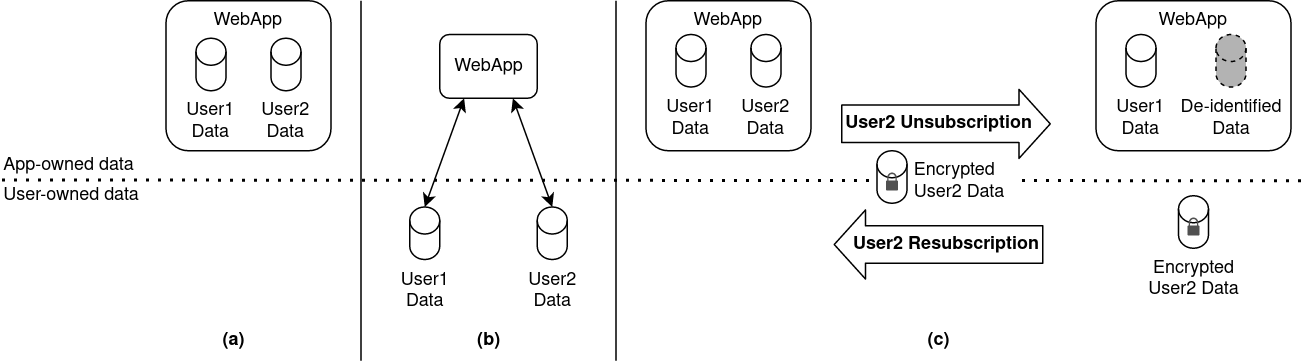
\includegraphics[width=\textwidth]{img/worlds}
%
%    \caption{\textbf{(a)} The current web application paradigm, in which applications maintain and
%    own user data; \textbf{(b)} A paradigm that decouples user data from web applications, giving users ownership of their data;
%    \textbf{(c)} \name, which allows users to switch between privacy-preserving unsubscribed mode (right) and identity-revealing subscribed mode (left).}
%    \label{fig:world}
%\end{figure*}
%
Web applications today own, store, and sell user data, often without the user's knowledge or
explicit consent~\cite{nytimes:fb, npr:data}. This both violates users' right for privacy, and has
dangerous consequences for both users and application developers as data leaks lead to loss of
livelihoods and lawsuits~\cite{breach:amazon,breach:twitter, breach:fb, breach:marriott,
breach:quora}.
%Granting web applications complete ownership of personal data clearly fails to
%protect users' privacy.

Although users want stronger privacy, completely decoupling user data from applications results in a
potentially even less desirable world. While possible~\cite{solid, amber, w5, blockstack, bstore}, such a
model hinders service-side computation and application performance, and requires users to manage
long-time security and storage of their data, leading to a lack of adoption in practice (Section~\ref{sec:related}).

This paper proposes \name, a new paradigm that grants users flexible privacy when using web
applications, balancing users' desire for privacy with their desire for application utility. In
\name, users subscribe to applications by granting a time-limited lease to their data, with the
provision that the application may retain only de-identified information once the user unsubscribes.
Users flexibly switch between a privacy-preserving unsubscribed mode and an identity-revealing
subscribed mode at any time without permanently losing their data. \name contrasts
with the current web application paradigm for data ownership, in which applications have complete
ownership, and the other extreme in which the user has complete data ownership.% (see Figure~\ref{fig:world}).

\name benefits users: they can choose privacy at any time, without
permanently losing their accounts or affecting the utility of the applications for others.  Just as
importantly, \name also benefits application developers. Recent laws such as the
European Union's General Data Protection Regulation (GDPR)~\cite{eu:gdpr} and California's Consumer
Privacy Act (CCPA)~\cite{ca:privacy-act} codify users' rights to data ownership, granting users the
right to request erasure of information related to them. Supporting \name enables
applications to comply with these legal mandates, while still allowing its departing users to easily
come back: if applications must let users leave, it is in their best interest to make it easy for
them to return.

Furthermore, applications can continue to operate using their current revenue model, maintaining
performance, reliability, and utility for their users.  Because applications retain use of
subscribed users' data, and de-identified data of unsubscribed users, applications optimize the
amount of data available to generate profit and provide utility for subscribed users. The
application holds only identifying data for subscribed users, reducing the amount of
compromising data in the system to only those users who have actively agreed to temporarily give up
their privacy.

Realizing \name poses a number of technical challenges.
Unsubscription and resubscription requires complex and fragile data transformations: developers must
selectively retain unsubscribed users' data for legal or application purposes while properly
de-identifying this data, a non-trivial task in the face of subtle inference attacks (\eg tags on a
user's post can identify the user). De-identification and data removal needs to be reversible,
allowing the user to resubscribe at any time to their last-known subscribed state.

To make \name a reality, we model application data as an abstract \emph{entity graph}, and
represent unsubscription and resubscription as transformations of this graph.
\emph{Ghost entities} allow transformations to achieve both data retention and de-identification,
and declarative \emph{ghost policies} specify reversible transformations upon unsubscription.
We design and implement \sys, a practical system that systematically automates this transformation for new and existing applications, helping developers realize the \name paradigm without onerous labor.
%that takes a developer-specified unsubscription policy for the application's entity
%graph, and ensures that
%that requires developers only to specify an abstract unsubscription policy on the
%helps developers of databased-backed web applications automatically achieve correct, privacy-compliant user unsubscription and
%resubscription without onerous labor.
\fi
